\section{Základní struktura na tranzistorové úrovni }
-logické obvody v unipolárních technologiích - invertor, AND, NAND, NOR, OR.

\subsection{Invertor}
   \begin{figure}[h]
   \begin{center}
     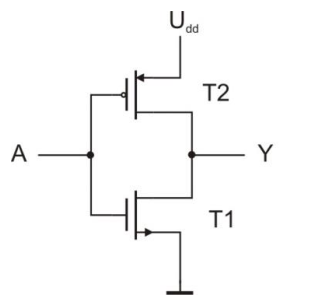
\includegraphics[scale=0.6]{images/INVCMOS.png}
   \end{center}
   \caption{Funkce INV v CMOS technologii}
  \end{figure}
   \pagebreak
\subsection{NAND}
   \begin{figure}[h]
   \begin{center}
     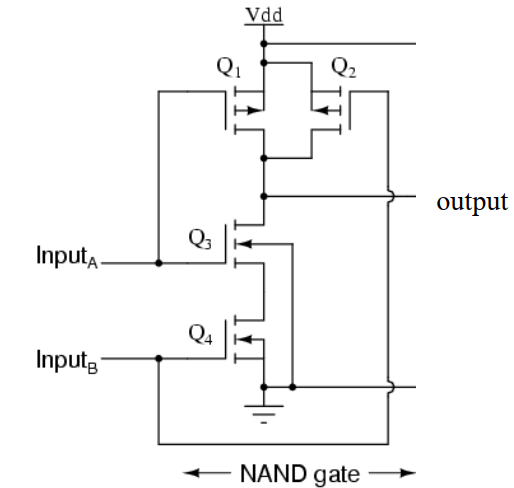
\includegraphics[scale=0.6]{images/NANDCMOS.png}
   \end{center}
   \caption{Funkce NAND v CMOS technologii}
  \end{figure}
 \pagebreak
\subsection{AND}
   \begin{figure}[h]
   \begin{center}
     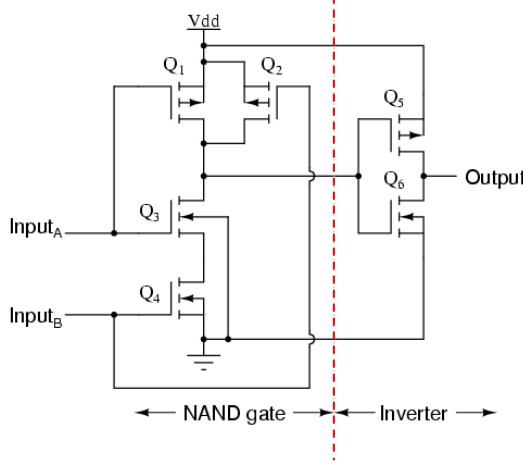
\includegraphics[scale=0.6]{images/ANDCMOS.png}
   \end{center}
   \caption{Funkce AND v CMOS technologii}
  \end{figure}
 \pagebreak
\subsection{NOR}
   \begin{figure}[h]
   \begin{center}
     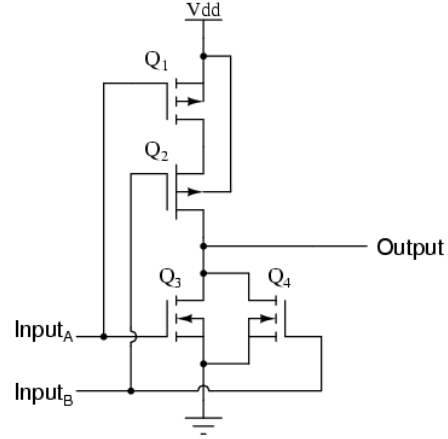
\includegraphics[scale=0.6]{images/NORCMOS.png}
   \end{center}
   \caption{Funkce NOR v CMOS technologii}
  \end{figure}
   \pagebreak
\subsection{OR}

   \begin{figure}[h]
   \begin{center}
     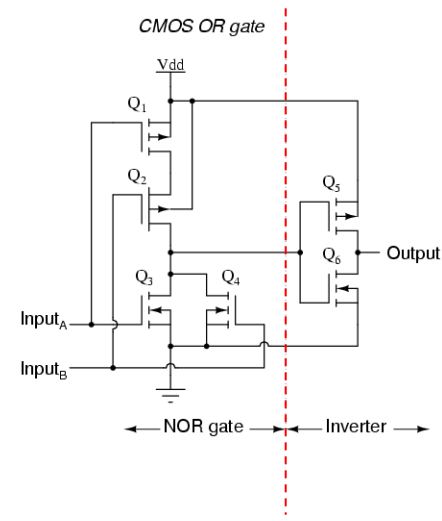
\includegraphics[scale=0.6]{images/ORCMOS.png}
   \end{center}
   \caption{Funkce OR v CMOS technologii}
  \end{figure}